

\begin{figure}[t!]
  \centering
  \begin{minipage}[t]{0.49\textwidth}
    \centering
    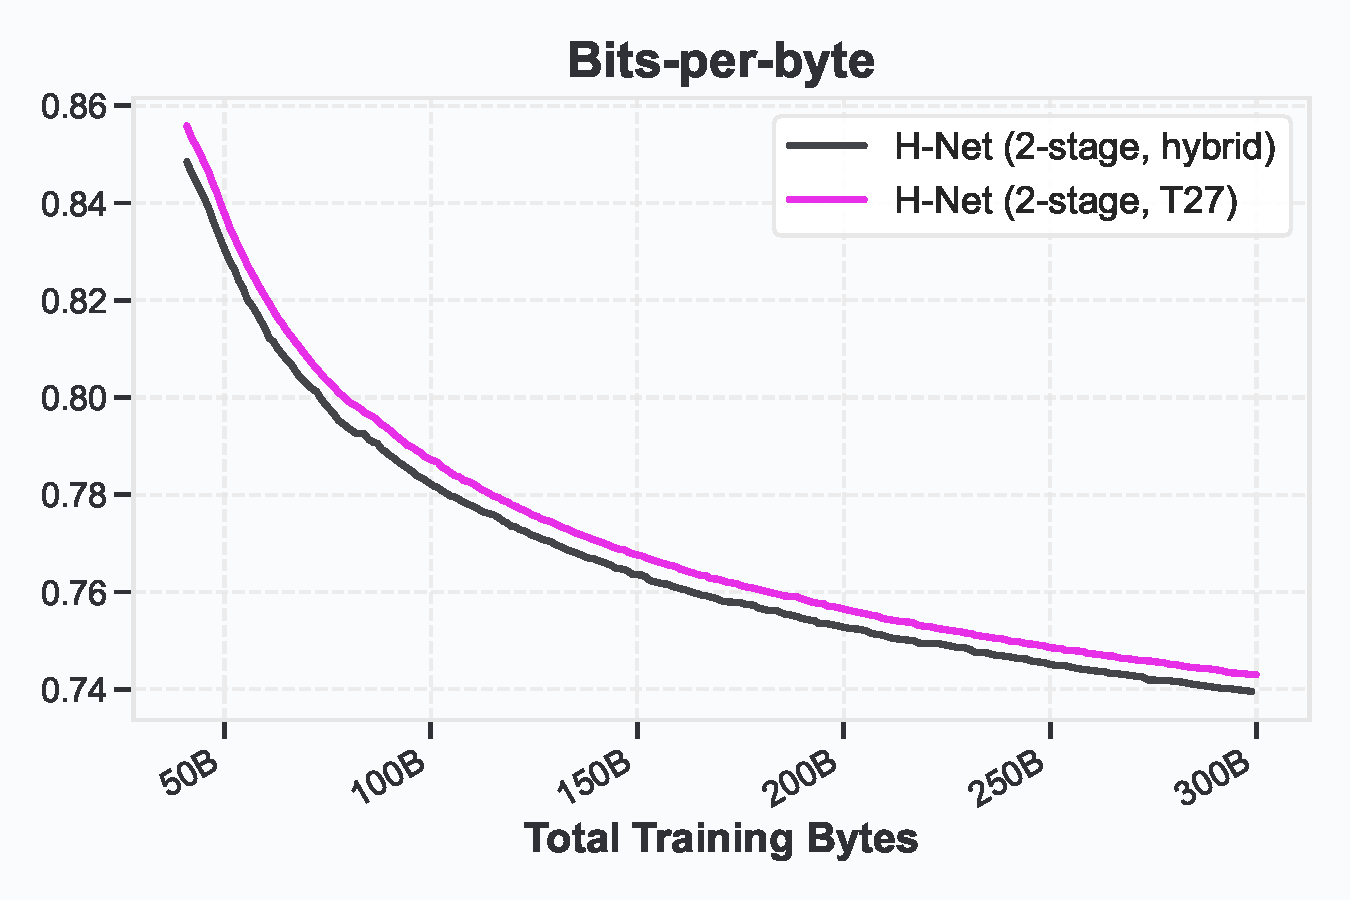
\includegraphics[width=1.0\linewidth]{fig_img/hybrid.pdf}
    \captionof{figure}{\textbf{Hybrid main network.} Bits-per-byte during the stable phase of training, for \model{} (2-stage) with Transformer main stage and with hybrid main stage.
    The hybrid main stage scales better, similar to findings for standard token-based language models. This finding suggests that design principles for isotropic (tokenized) models can carry over to choices of the main network.}
    \label{fig: hybrid}
  \end{minipage}
  \hfill
  \begin{minipage}[t]{0.49\textwidth}
    \centering
    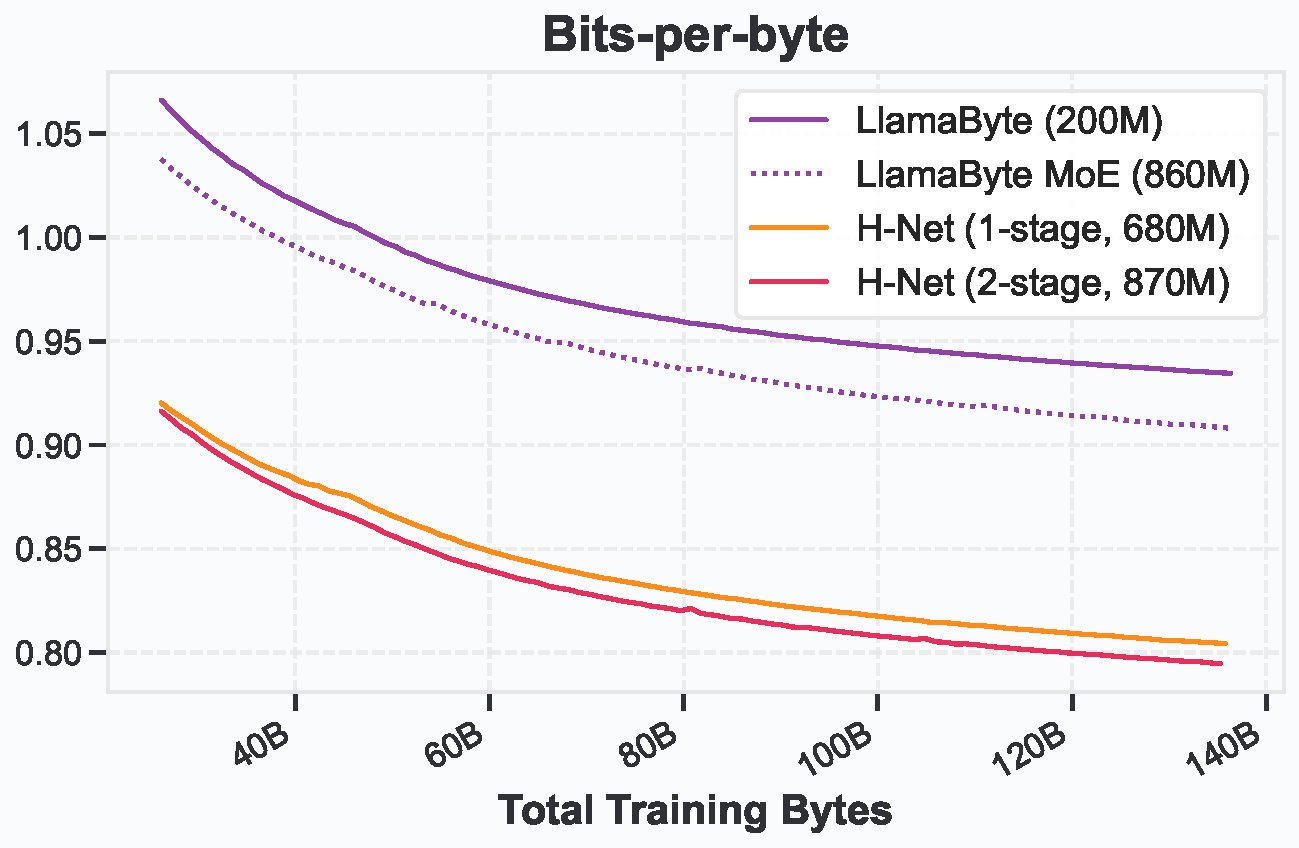
\includegraphics[width=1.0\linewidth]{fig_img/abl_moe.pdf}
    \captionof{figure}{\textbf{Comparison to Mixtures-of-Experts.} Bits-per-byte comparison of \model{} (both 1-stage and 2-stage) to LlamaByte-MoE, which is a FLOPs-matched MoE model that uses a similar number of parameters as \model{} (2-stage). Both \model{}s perform much better than LlamaByte-MoE, implying that \model{}'s capabilities do not just come from  sparsity.}
    \label{fig: moe}
  \end{minipage}
\end{figure}